\documentclass[../main.tex]{subfiles}

\begin{document}
\textbf{Problem:} Find a straight line $L$ that is tangent to a curve $C$ at a point $P$.

\textsf{``For simplicity, restrict ourselves to curves which are graphs of functions.''}

\textbf{How do we define the tangent line to a curve?}
\begin{figure}[htbp]
    \centering
    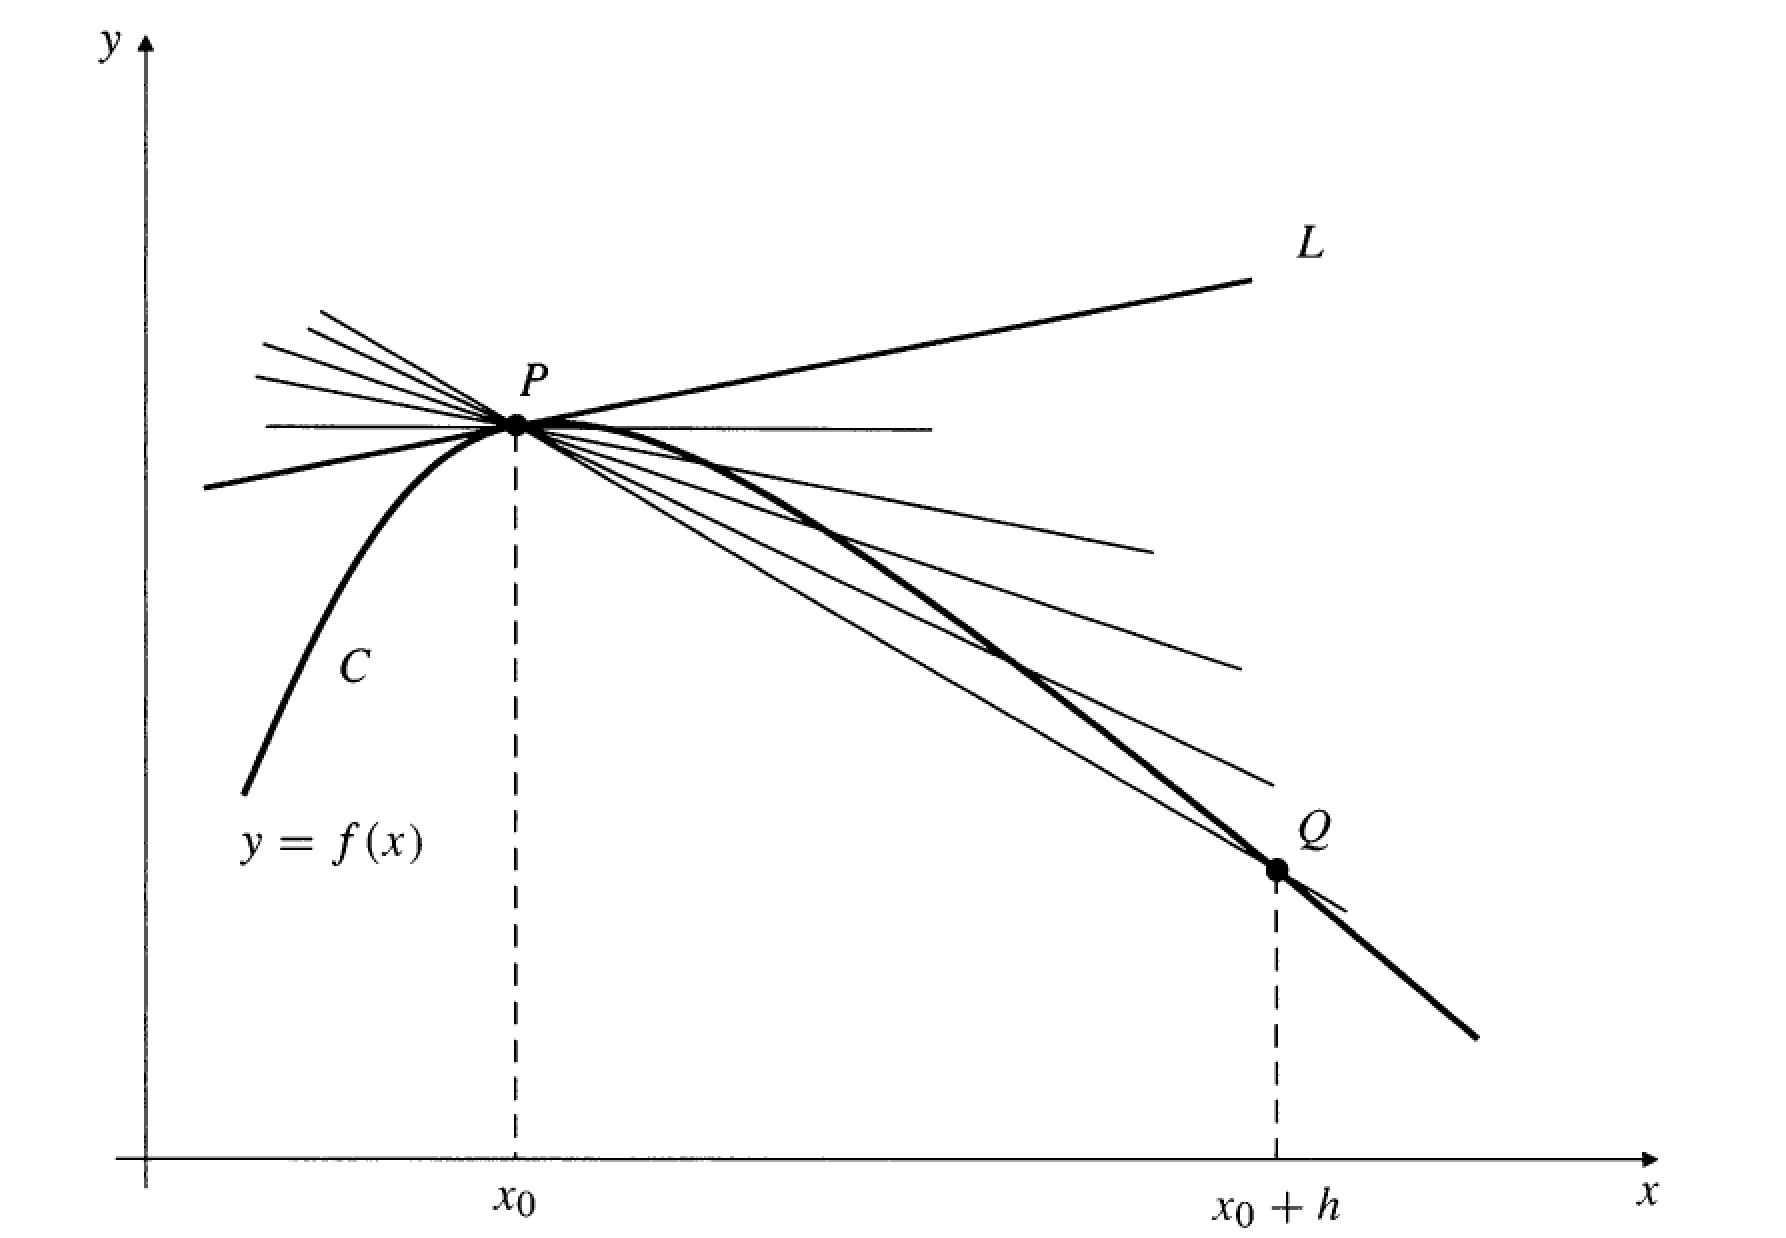
\includegraphics[scale=0.3]{adams-2-1-fig4}
    \caption{caption}
    \label{fig:label}
\end{figure}
The slope of the line PQ is
\[
    \dfrac{f(x_0 + h) - f(x_0)}{h}.
\]

\begin{definition}
    Suppose $f$ is cts at $x=x_0$ and
    \[
        \Lim{h}{0} \dfrac{f(x_0 + h) - f(x_0)}{h} = m
    \]
    If the limit exists, then the line with equation
    \[
        y = m(x - x_0) + f(x_0)
    \]
    is called \textbf{the tangent line} to the graph of $y=f(x)$ at $P = (x_0, f(x_0))$.
    If the limit does not exist and $m = \infty$ or $m = -\infty$ then the tangent line is the vertical line $x=x_0$.
    If the limit does not exist and is not $\pm \infty$ then there is no tangent line at $P$.
\end{definition}

\begin{example}
    Find an equation of the tangent line to the curve $y = x^2$ at $(1, 1)$.
\end{example}
\begin{solution}
    \[
        m = \Lim{h}{0} \dfrac{f(1+h)-f(1)}{h} = 2.
    \]
    And an equation is $y=2(x-1)+1$
\end{solution}
\begin{example}
    Find an equation of the tangent line to the curve $y = x^{1/3} = \sqrt[3]{x}$ at the origin.
\end{example}
\begin{solution}
    The slope of the tangent line is
    \[
        m = \Lim{h}{0} \dfrac{h^{1/3}}{h} = \infty.
    \]
    So the tangent line is a vertical line $x=0$ (in other words the y-axis).
    \begin{figure}[H]
        \centering
        % p = Plot[CubeRoot[x], {x, -1, 1}, Ticks -> None,
        %   PlotStyle -> {Thick, Black}, ImageSize -> 50]
        % Export["cuberoot.pdf", p]
        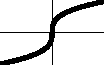
\includegraphics[scale=1]{cuberoot}
        \caption{$y=x^{1/3}$}
    \end{figure}
\end{solution}

\begin{example}
    Does $f(x) = x^{2/3}$ have a tangent line at $(0, 0)$?
\end{example}
\begin{solution}
    The limit of the difference quotient is undefined at $0$since the right limit is $\infty$ while the left limit is $-\infty$. Hence the graph has no tangent line at $(0, 0)$.
    \begin{figure}[H]
    % p = Plot[CubeRoot[x]^2, {x, -1, 1}, Ticks -> None,
    %   PlotStyle -> {Thick, Black}, ImageSize -> 50]
    % Export["sqrofcuberoot.pdf", p]
        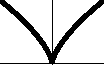
\includegraphics[scale=1]{sqrofcuberoot}
        \caption{$y=x^{2/3}$}
    \end{figure}

    \textsf{``We say that this curve has a cusp at the origin. A cusp is an infinitely sharp point. If you were traveling along the curve, you would have to stop and turn 180$^{\circ}$ at the origin.''}
\end{solution}

\begin{example}
    Does $f(x) = \abs{x}$ have a tangent line at $(0, 0)$?
\end{example}

\begin{solution}
    The difference quotient is $\dfrac{\abs{h}}{h}$ which has right limit $1$ and left limit $-1$ at $h=0$.
    \begin{figure}[H]
    % p = Plot[Abs[x], {x, -1, 1}, Ticks -> None,
    %   PlotStyle -> {Thick, Black}, ImageSize -> 50]
    % Export["absvalue.pdf", p]
        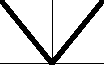
\includegraphics[scale=1]{absvalue}
        \caption{$y=\abs{x}$}
    \end{figure}
\end{solution}

\end{document}